\documentclass[table]{beamer}
\usepackage[utf8]{inputenc}
\usepackage[squaren]{SIunits}
\usepackage{varwidth,setspace}
\usepackage{tikz}
\usetikzlibrary{intersections,positioning,backgrounds,fit,matrix,shapes,calc,decorations.pathmorphing,decorations.text}
\usetheme{default}

\newcommand*{\mimg}[2]{\begingroup
\setbox0=\hbox{\includegraphics[height=#2]{#1}}\parbox{\wd0}{\box0}\endgroup}
\newcommand*{\rmimg}[2]{\begingroup
\setbox0=\hbox{\includegraphics[angle=90,origin=c,height=#2]{#1}}\parbox{\wd0}{\box0}\endgroup}
\newcommand*{\symok}[0]{\includegraphics[height=1em]{symbol_ok.pdf}}
\newcommand*{\symbad}[0]{\includegraphics[height=1em]{symbol_bad.pdf}}
\newcommand*{\symidk}[0]{{\bf\color{blue}\Large?}}

\setbeamertemplate{navigation symbols}{}%remove navigation symbols
\setbeamertemplate{footline}{\hspace*{.5cm}\scriptsize{\hfill\raisebox{1mm}{\insertframenumber}\hspace*{.5cm}}}

\setlength{\tabcolsep}{0.5mm}

\title{Exploring the dark universe with the Atacama Cosmology Telescope}
\author{Sigurd Kirkevold Næss}
\institute{Subdepartment of astrophysics, Oxford University}
\date{October 13th, 2014}

\begin{document}

\begin{frame}
	\titlepage
	\vspace{-1cm}
	\begin{center}
	%{\footnotesize The source code of this talk can be found at {\color[rgb]{0,0.7,0}https://github.com/amaurea/talk-bmode}}
	\end{center}
\end{frame}

\begin{frame}{The physics of CMB lensing}
	\begin{center}
		\begin{tikzpicture}
			\node at (0,0) {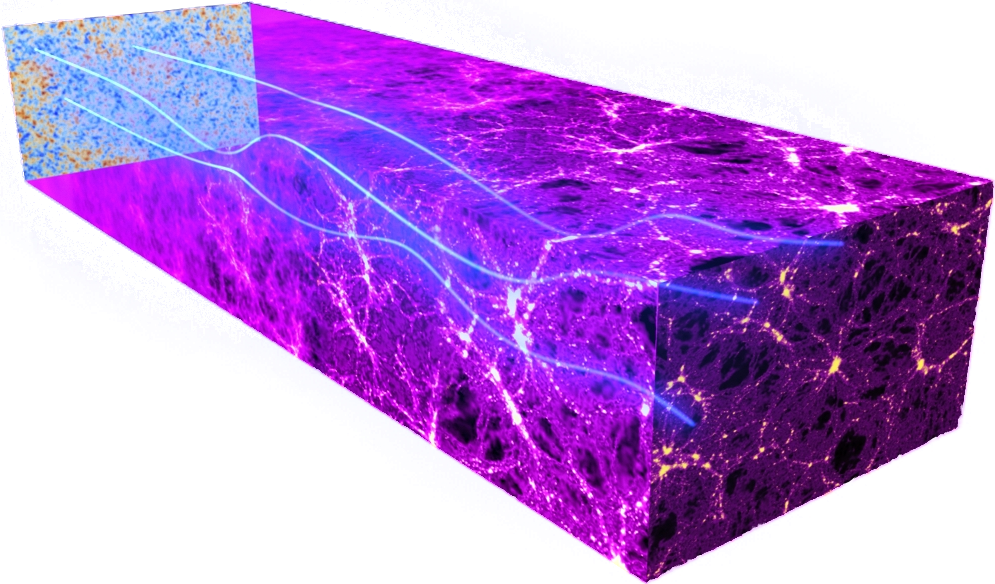
\includegraphics[width=\textwidth]{plots/Planck_gravitational_lensing_CMB_transparent.png}};
			\uncover<2->{\draw[thick,white,dashed] (-5,2.6) -- (2.4,-0.4);}
			\uncover<3->{\draw[thick,white,->] (2.4,-0.4) -- (2.8,-0.15);}
			\uncover<4->{\node[white] at (3.5,-0.5) {$\sim3$ arcmin};}
		\end{tikzpicture}

		{\footnotesize Credit: Planck, ESA}
	\end{center}
\end{frame}

\begin{frame}{Lensing distorts the CMB}
	\begin{center}
		\begin{tikzpicture}
			\only<1>{\node at (0,0) {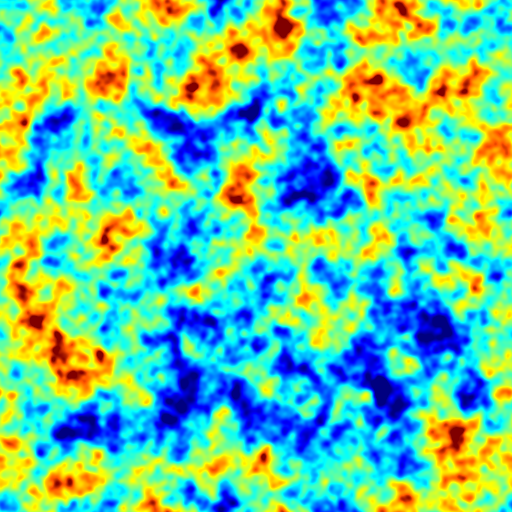
\includegraphics[height=7cm]{plots/maps/T.png}};}%
			\only<2>{\node at (0,0) {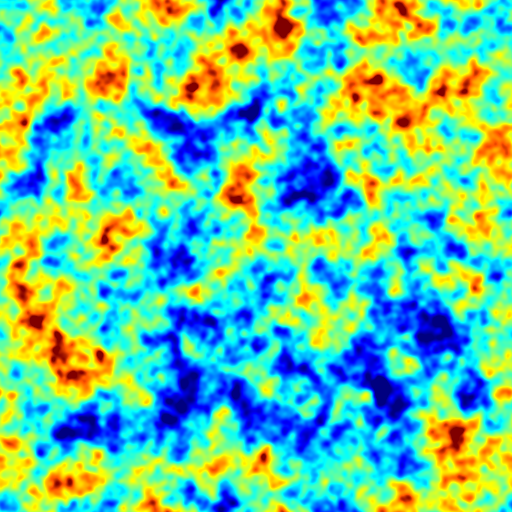
\includegraphics[height=7cm]{plots/maps/T.png}};}%
			\only<3>{\node at (0,0) {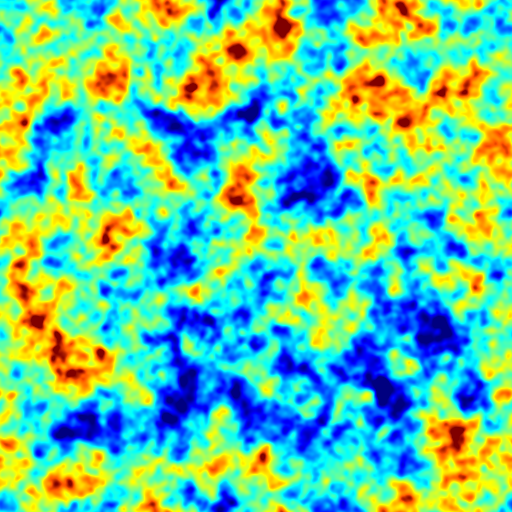
\includegraphics[height=7cm]{plots/maps/TlT.png}};}%
			\only<4-5>{\node at (0,0) {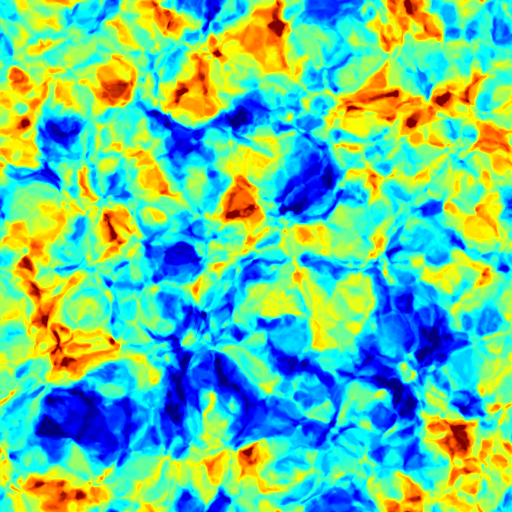
\includegraphics[height=7cm]{plots/maps/TsT.png}};}%
			\only<2-4>{\node at (0,0) {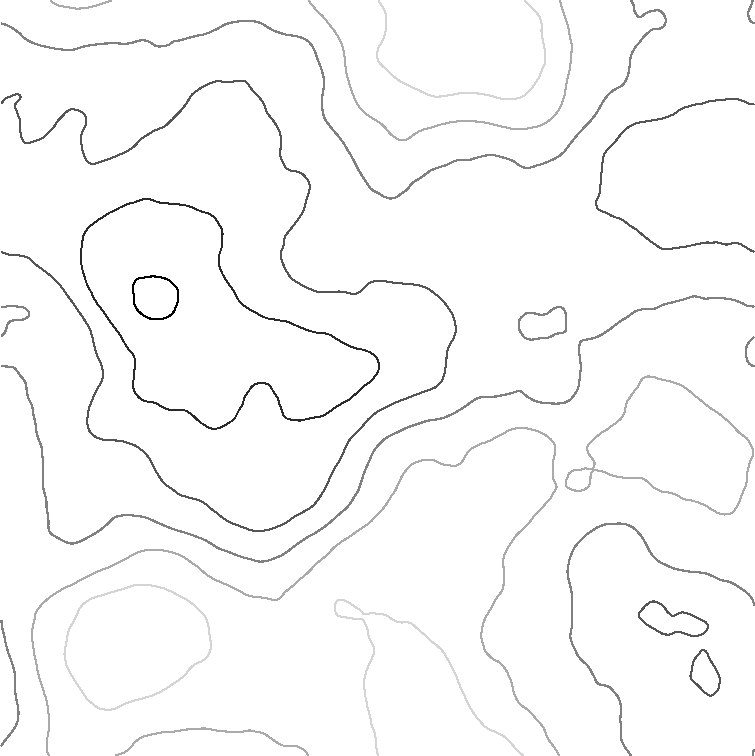
\includegraphics[height=7cm]{plots/maps/phi_contours.png}};}%
		\end{tikzpicture}

		\only<1>{Unlensed\uncover<0>{p}}%
		\only<2>{Gravitational potential}%
		\only<3>{Lensed\uncover<0>{p}}%
		\only<4>{Lensed x10\uncover<0>{p}}%
		\only<5>{Non-Gaussian\uncover<0>{p}}%
	\end{center}
\end{frame}

\begin{frame}{Lensing distorts the CMB Polarization}
	\begin{center}
		\hspace*{-3mm}
		\begin{tabular}{cc}
			{\bf Q} ($\pm 20\mu$K) & {\bf U} ($\pm 20\mu$K) \\
			\only<1>{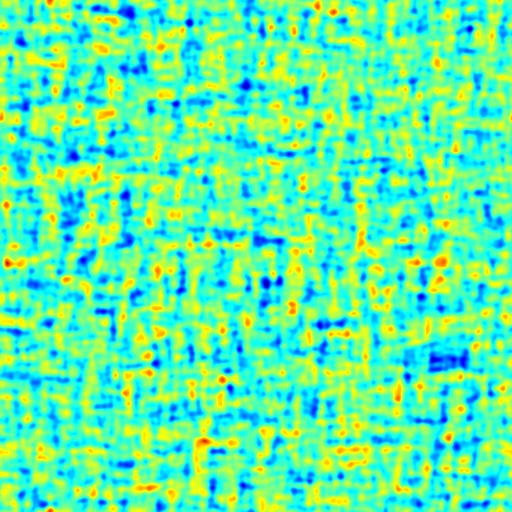
\includegraphics[height=5.5cm]{plots/maps/EBQ.png}}%
			\only<2>{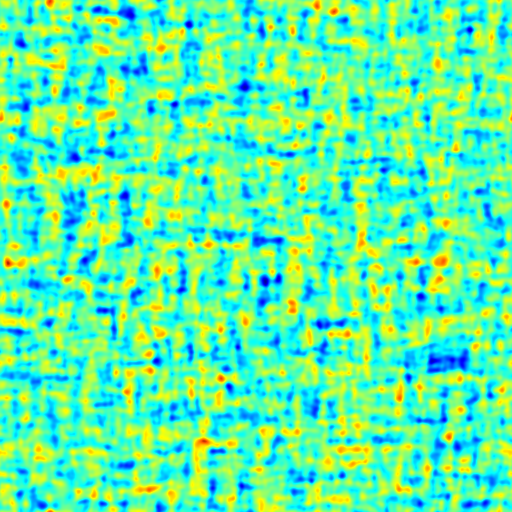
\includegraphics[height=5.5cm]{plots/maps/EBlQ.png}}%
			&
			\only<1>{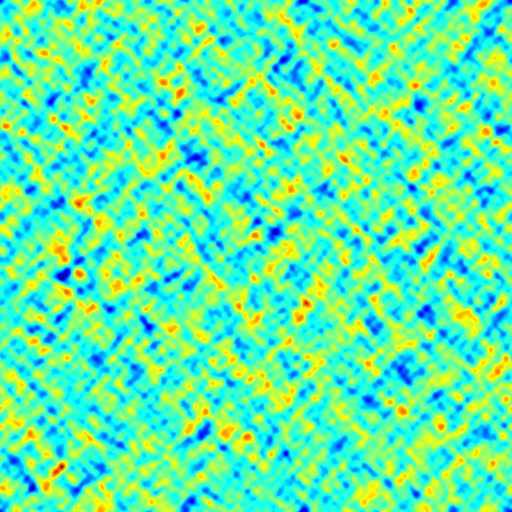
\includegraphics[height=5.5cm]{plots/maps/EBU.png}}%
			\only<2>{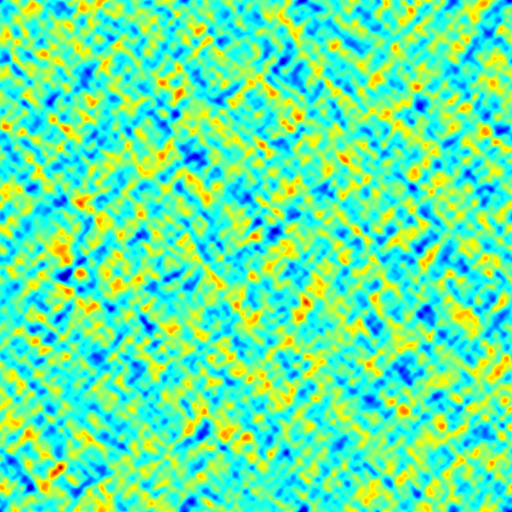
\includegraphics[height=5.5cm]{plots/maps/EBlU.png}}%
		\end{tabular}

		\only<1>{Unlensed}%
		\only<2>{Lensed}%
	\end{center}
\end{frame}

\begin{frame}{E, B and Q, U}
	\begin{center}
		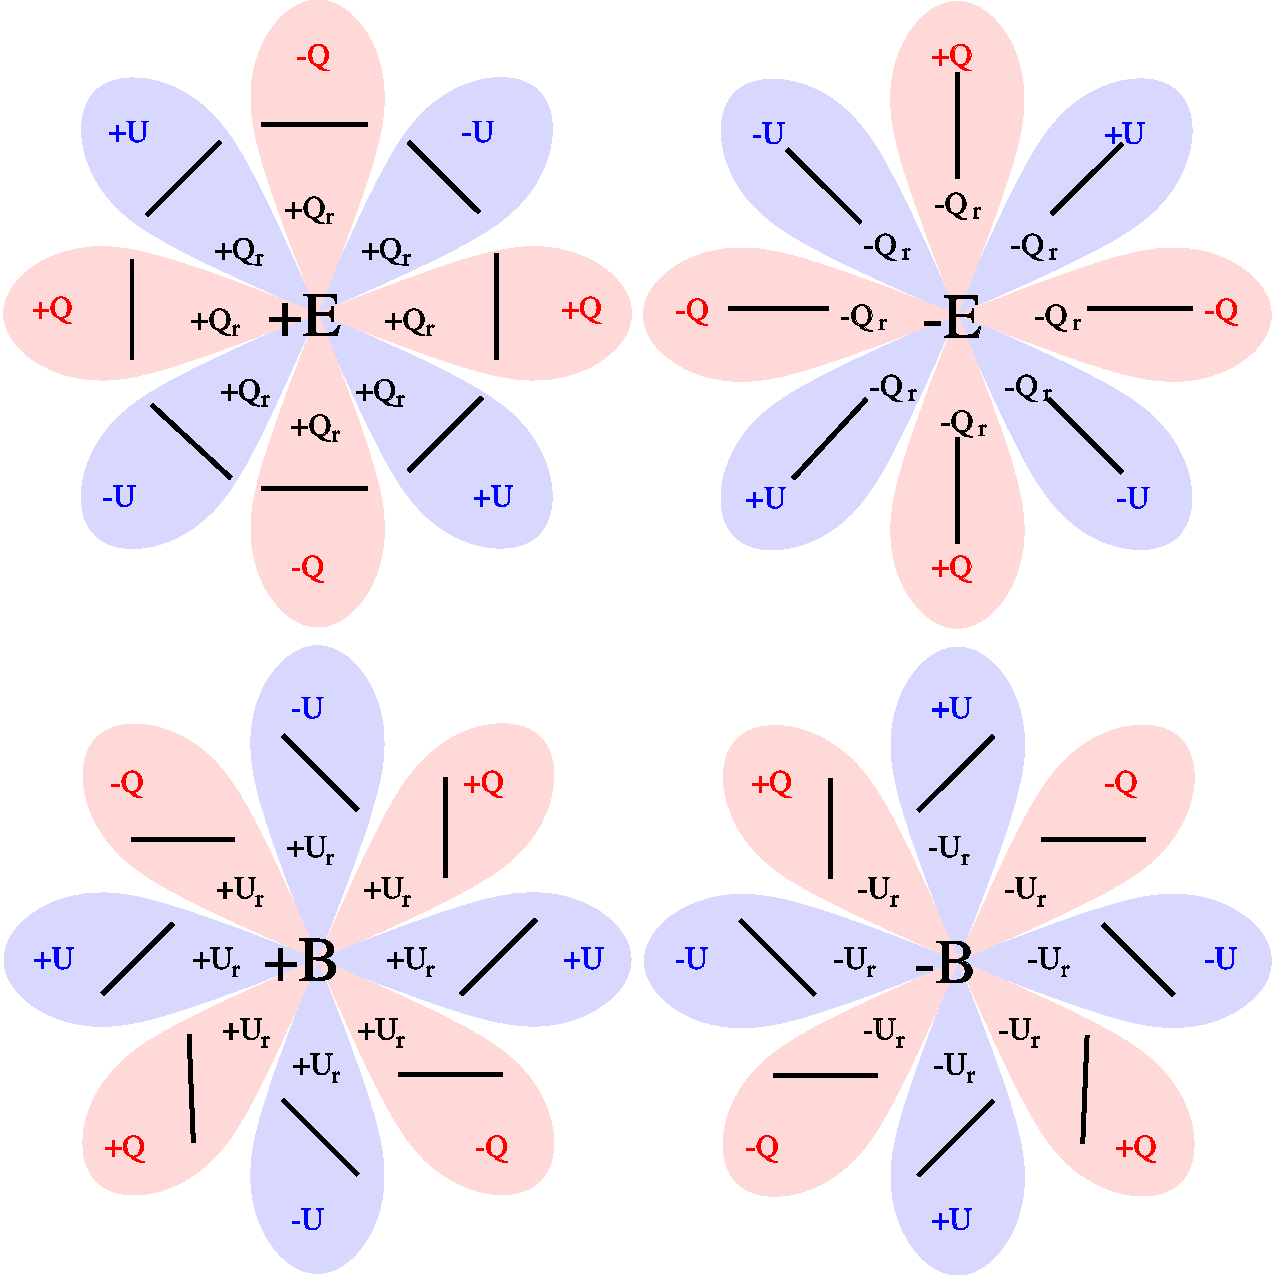
\includegraphics[height=8cm]{plots/EB_healpix.pdf}
	\end{center}
\end{frame}

\begin{frame}{E,B and Q, U}
	\begin{center}
		\only<1>{E and B result from quadrupole-convolutions of Q and U}%
		\only<2>{Reverse also holds}%

	\scalebox{1.7}{
		\begin{minipage}{5cm}
			\begin{align*}
				\only<1>{%
				E =& \rmimg{plots/queb_0.png}{1cm} \otimes Q + \mimg{plots/queb_2.png}{1cm} \otimes U \\
				B =& \mimg{plots/queb_1.png}{1cm} \otimes Q + \rmimg{plots/queb_3.png}{1cm} \otimes U}%
				\only<2>{%
				Q =& \rmimg{plots/ebqu_0.png}{1cm} \otimes E + \mimg{plots/ebqu_2.png}{1cm} \otimes B \\
				U =& \mimg{plots/ebqu_1.png}{1cm} \otimes E + \rmimg{plots/ebqu_3.png}{1cm} \otimes B}%
			\end{align*}
		\end{minipage}}
	\end{center}
\end{frame}

\begin{frame}{Lensing distorts E and B}
	\begin{center}
		\hspace*{-3mm}
		\begin{tabular}{cc}
			{\bf E} ($\pm 20\mu$K) & {\bf B} ($\pm 0.5\mu$K) \\
			\only<1>{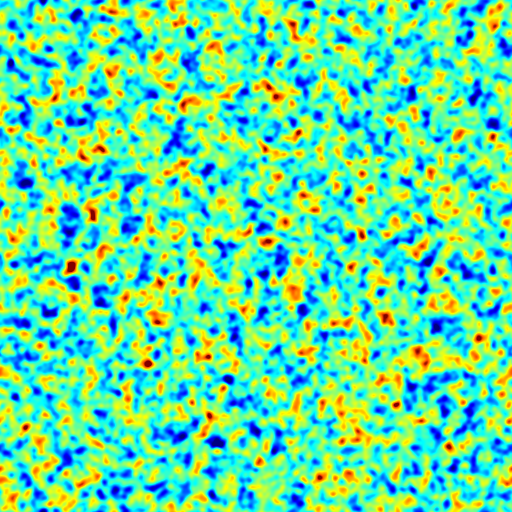
\includegraphics[height=5.5cm]{plots/maps/E.png}}%
			\only<2>{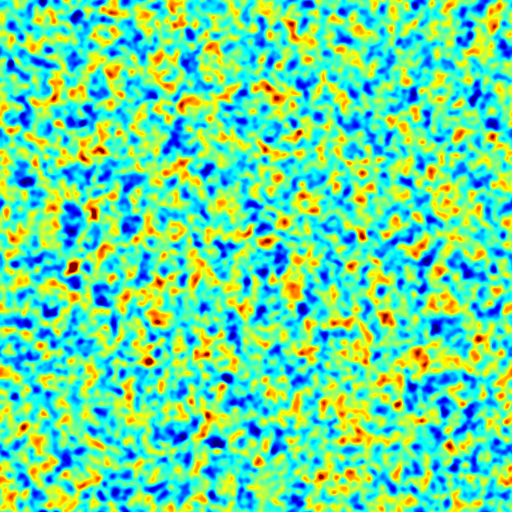
\includegraphics[height=5.5cm]{plots/maps/EBlE.png}}%
			&
			\only<1>{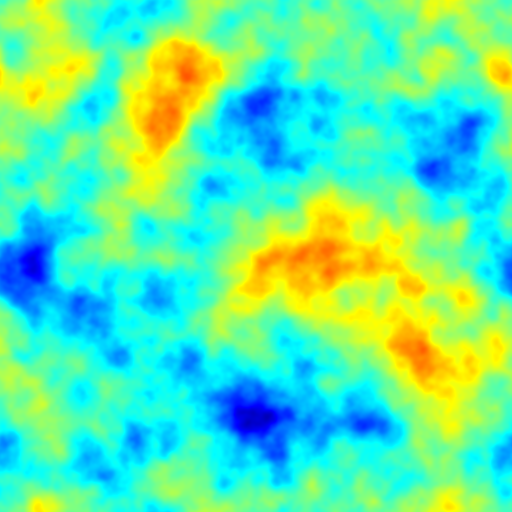
\includegraphics[height=5.5cm]{plots/maps/B.png}}%
			\only<2>{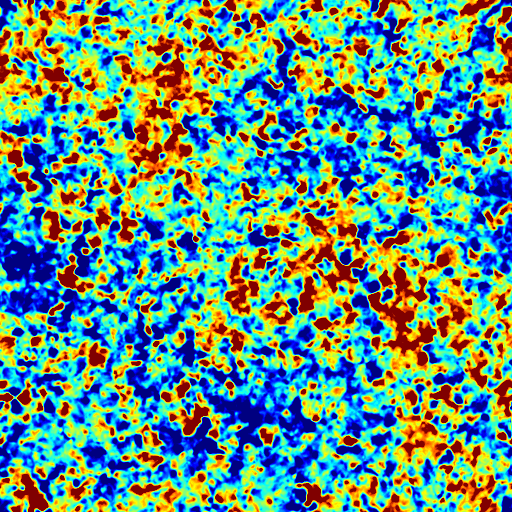
\includegraphics[height=5.5cm]{plots/maps/EBlB.png}}%
		\end{tabular}

		\only<1>{Unlensed}%
		\only<2>{Lensed}%
	\end{center}
\end{frame}

\begin{frame}{Lensing distorts the power spectra}
	\begin{center}
		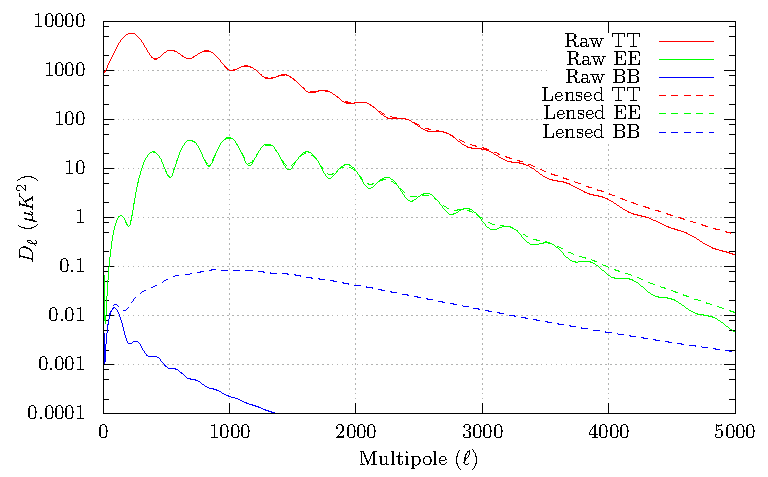
\includegraphics[width=\textwidth]{plots/spectra.pdf}
	\end{center}
\end{frame}

\begin{frame}{Disentangling CMB and lensing}
	\begin{center}
		\begin{itemize}
			\item Lensing correlates previously uncorrelated multipoles
				\begin{tabular}{lll}
					Before & $\langle T(\mathbf{l}_1)T(\mathbf{l}_2)\rangle = 0$ & for $\mathbf{l}_1 \ne \mathbf{l}_2$ \\
					After &  $\langle T(\mathbf{l}_1)T(\mathbf{l}_2)\rangle \propto \phi(\mathbf{l}_1+\mathbf{l}_2)$ & for $\mathbf{l}_1 \ne \mathbf{l}_2$
				\end{tabular}
			\item \uncover<2->{Use cross-correlations to reconstruct lensing potential}
				\begin{tikzpicture}
					\node at (0,0) {%
						$\begin{aligned}
							\uncover<3->{%
							\begin{matrix}
								\textrm{\tiny lensed T}\left\{\mimg{plots/maps/TlT.png}{2cm}\right. \\
								\textrm{\tiny lensed E}\left\{\mimg{plots/maps/EBlE.png}{2cm}\right. \\
								\textrm{\tiny lensed B}\left\{\mimg{plots/maps/EBlB.png}{2cm}\right.
							\end{matrix}}
							\uncover<4->{%
							\rightarrow
							\underbrace{\mimg{plots/maps/phi.png}{2cm}}_{\textrm{\tiny lensing potential }\phi}}
							\uncover<5->{%
							\rightarrow
							\begin{matrix}
								\left.\mimg{plots/maps/T.png}{2cm}\right\}\textrm{\tiny true T} \\
								\left.\mimg{plots/maps/E.png}{2cm}\right\}\textrm{\tiny true E} \\
								\left.\mimg{plots/maps/B.png}{2cm}\right\}\textrm{\tiny true B}
							\end{matrix}}
					\end{aligned}$};
					\uncover<6->{\draw[thick,red] (0.15,-0.25) circle (1.62);}
			\end{tikzpicture}
		\end{itemize}
	\end{center}
\end{frame}

\begin{frame}{Pure CMB is degenerate}
	\begin{center}
		\vspace{-10mm}
		\begin{tikzpicture}
			\node at ( 4.15,0.12) {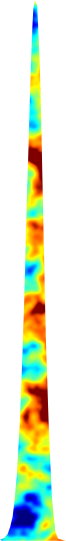
\includegraphics[height=4.2cm]{plots/cmb_slice.png}};
			\node at ( 0.00,0.00) {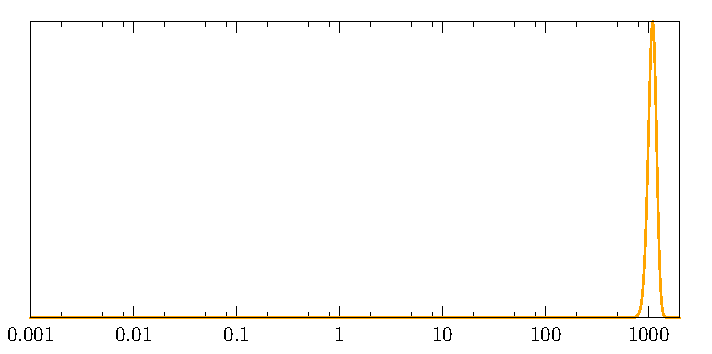
\includegraphics[width=10cm]{plots/z_cmb.pdf}};
			\node[orange] at (4.15,2.40) {CMB};
			\node at (-5.20,0.20) {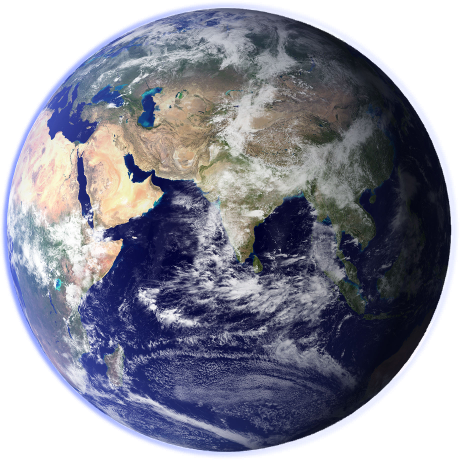
\includegraphics[height=1.0cm]{plots/earth.png}};
			\uncover<14->{%
			\node at ( 0.00,0.00) {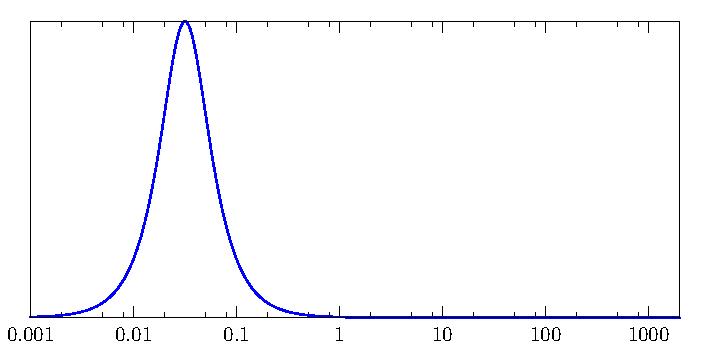
\includegraphics[width=10cm]{plots/z_sn.pdf}};
			\node[blue] at (-2.40,2.40) {SN};}
			\uncover<15->{%
			\node at ( 0.00,0.00) {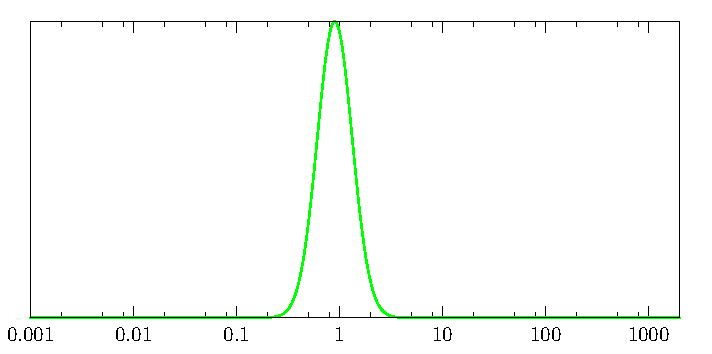
\includegraphics[width=10cm]{plots/z_bao.pdf}};
			\node[green] at (-0.32,2.40) {BAO};}
			\uncover<18->{%
			\node at ( 0.00,0.00) {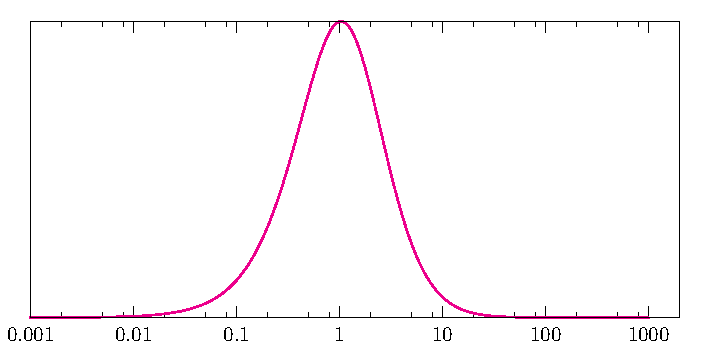
\includegraphics[width=10cm]{plots/z_lens.pdf}};
			\node[magenta,align=center] at (-0.24,0.00) {CMB\\Lensing};}

			\uncover<2-11>{%
			\draw[thick,red] (4.15,0.26) ellipse (0.4 and 2.5);}
			\uncover<3-11>{%
			\draw[ultra thick,red,<->] (-4.2,2.4) -- (3.6,2.4);
			\node[red] at (0.0,2.7) {$d_A$};}
			\uncover<4-11>{%
			\node[blue,scale=2] at (0,0.2) {\Huge ?};}

			\node at (0,-4) {$\begin{aligned}
				\uncover<5->{\mimg{plots/maps/degen1.png}{2cm}}
				\uncover<6->{\xrightarrow{-\Omega_\Lambda}}
				\uncover<7->{\mimg{plots/maps/degen2.png}{2cm}}
				\uncover<8->{\xrightarrow{+t_0}}
				\uncover<9->{\mimg{plots/maps/degen3.png}{2cm}}
				\uncover<10->{\xrightarrow{+\Omega_k}}
				\uncover<11->{\mimg{plots/maps/degen1.png}{2cm}}
				\end{aligned}$};

			\uncover<12>{\node[fill=white,align=center] at (0,-1.5) {
				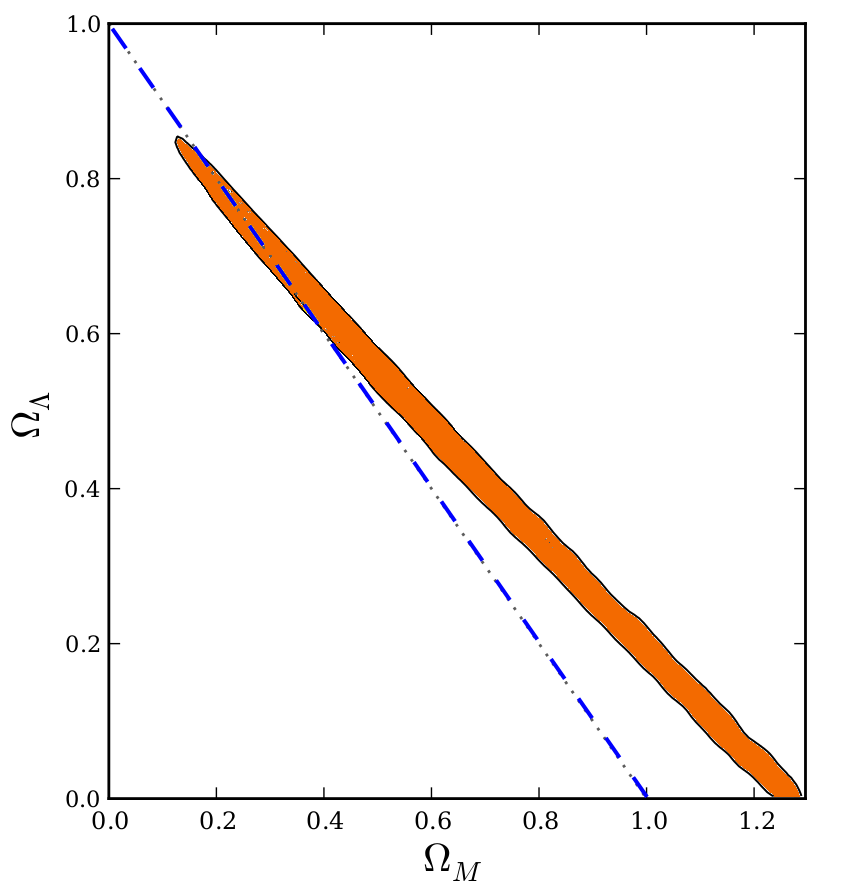
\includegraphics[height=7.5cm]{plots/cmb_nolens_degen.png}\\
				{\footnotesize Modified from Sherwin et al. 2011 \uncover<0>{g}}};}
			\uncover<16>{\node[fill=white,align=center] at (0,-1.5) {
				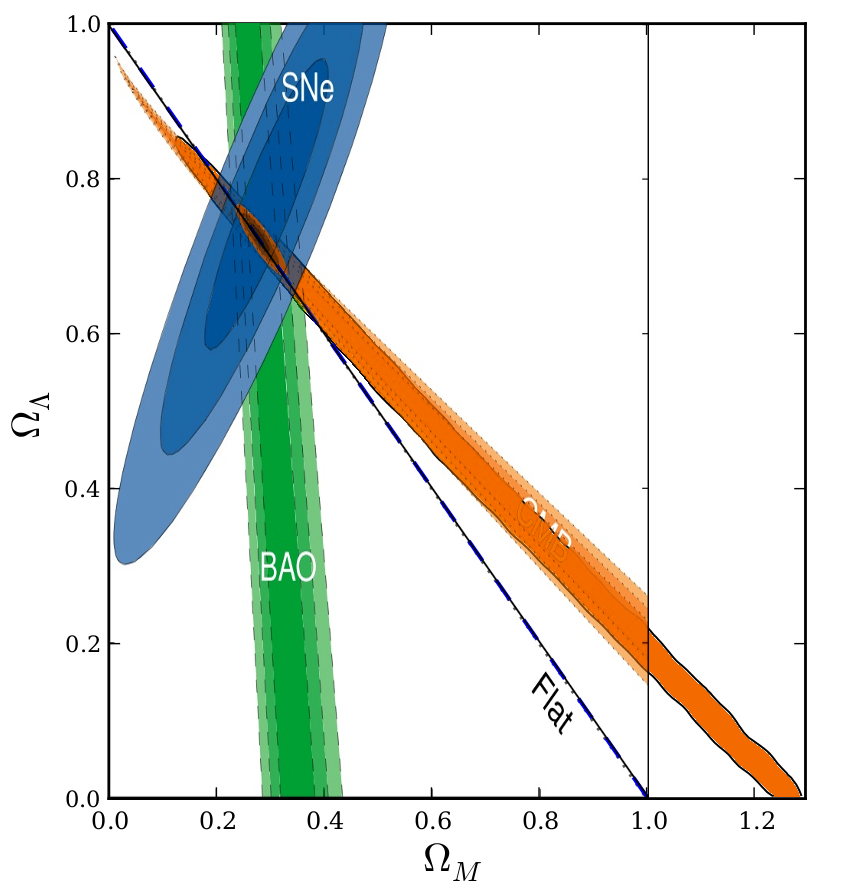
\includegraphics[height=7.5cm]{plots/cmb_nolens_sn_bao.png}\\
				{\footnotesize Modified from Supernova Cosmology Project 2010}};}

		\end{tikzpicture}
	\end{center}
\end{frame}

\begin{frame}{CMB lensing vs. other probes}
	\begin{itemize}
		\item Very clean
		\item (Mostly) linear physics
		\item Cannot split into redshift bins
	\end{itemize}
\end{frame}

\begin{frame}{3 main things to do with CMB lensing}
	\begin{center}
		\vspace{-0.5cm}%
		\hspace*{-0.7cm}%
		\begin{tikzpicture}
			\node[anchor=north,rounded corners,fill=red!10,  text height=7cm,text width=3.5cm] at (0,0) {};
			\node[anchor=north,rounded corners,fill=green!10,text height=7cm,text width=3.5cm] at (4,0) {};
			\node[anchor=north,rounded corners,fill=blue!10, text height=7cm,text width=3.5cm] at (8,0) {};

			\node[anchor=north] at (0,0) {
				\hspace*{-4mm}
				\begin{minipage}{4cm}
					\begin{center}
					{\large Power spectrum}
					\begin{itemize}
						\item Use directly as cosmological probe
						%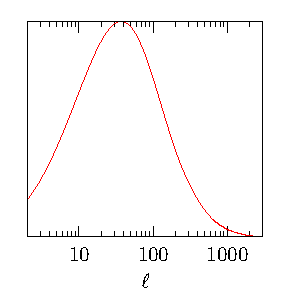
\includegraphics[height=2cm]{plots/cphi_small.pdf}
						% Replace with Planck neutrino mass phi spectrum plot from blake talk
						\item $\Omega_\Lambda$, $\sum m_\nu$, \ldots
						\item Astrophys.-independent dark energy measurement
					\end{itemize}
					\end{center}
				\end{minipage}
			};

			\node[anchor=north] at (4,0) {
				\hspace*{-4mm}
				\begin{minipage}{4cm}
					\begin{center}
					{\large Cross-correlation}
					\begin{itemize}
						\item Improve CMB lensing est.
						\item Use CMB lens. to calibrate others
						\item Result: Bias-free DM dist. for each z
						\item Bonus: Measure galaxy bias
					\end{itemize}
					\end{center}
				\end{minipage}
			};

			\node[anchor=north] at (8,0) {
				\hspace*{-4mm}
				\begin{minipage}{4cm}
					\begin{center}
					{\large Imaging}
					\begin{itemize}
						\item Map the lensing field
						\item Delensing for B-modes
						\item Check isotropy etc.
					\end{itemize}
					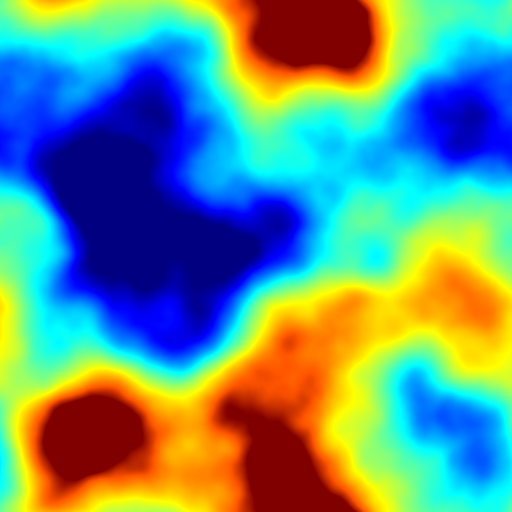
\includegraphics[height=3cm]{plots/maps/phi.png}
					\end{center}
				\end{minipage}
			};
		\end{tikzpicture}
	\end{center}
\end{frame}

\begin{frame}{Uses of CMB lensing 1: Power spectrum}
	\begin{itemize}
		\item<2-> Power smoothing in high-l $C_\ell^{TT}$
		\item<5-> Power excess in $C_\ell^{BB}$
		\item<8-> Power spectrum of lensing potential itself
		\item<11-> Phases not needed - large area can compensate for sensitivity
		\item<12-> Clean probe of $\Omega_\Lambda$, $\sum m_\nu$, $\ldots$
	\end{itemize}
	\hspace*{-1cm}
	\begin{tikzpicture}
		\uncover<3-5>{%
		\node at (0,0) {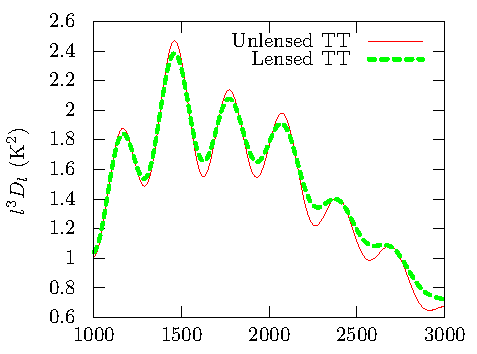
\includegraphics[height=4cm]{plots/excess_TT.pdf}};}
		\uncover<4-5>{%
		\node at (5.5,0) {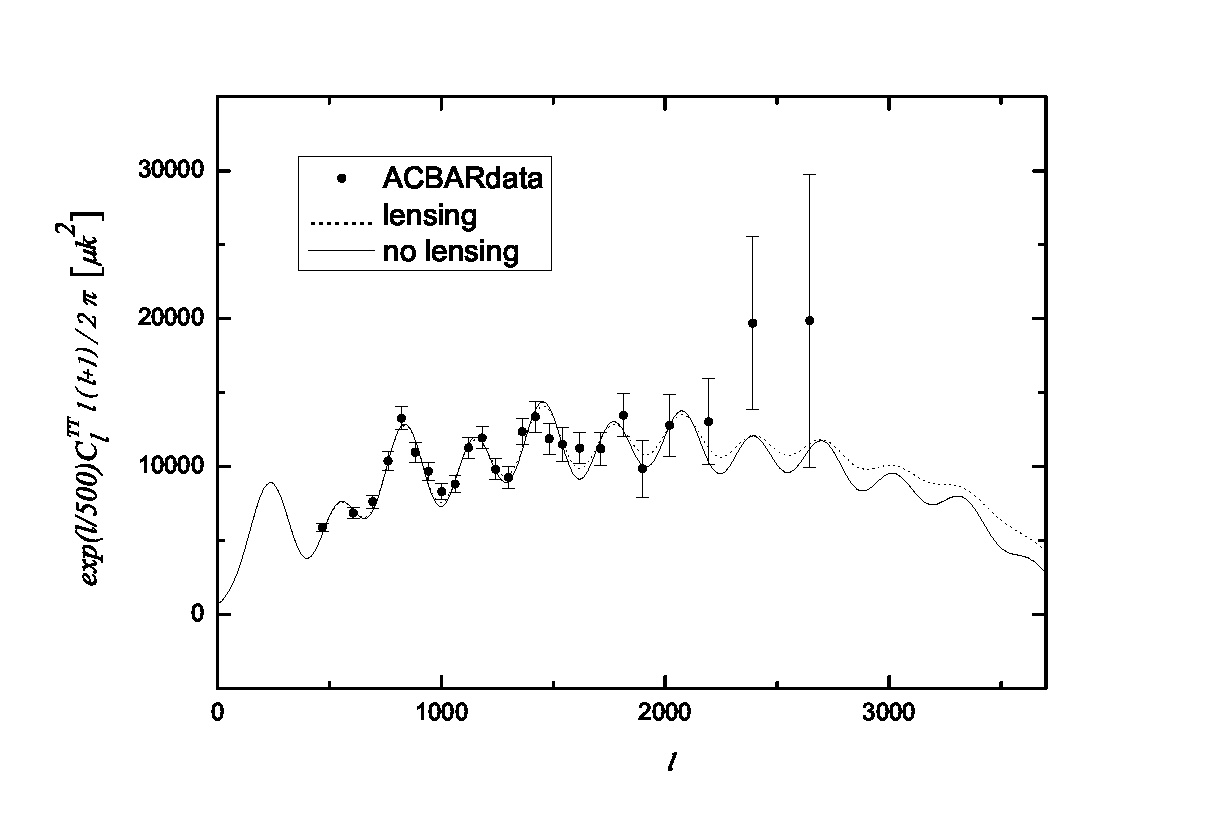
\includegraphics[height=4cm,clip,trim=20mm 11mm 10mm 9mm]{plots/acbar.pdf}};
		\node at (5.5,-1) {ACBAR 2008 $3\sigma$};}

		\uncover<6-8>{%
		\node at (0,0) {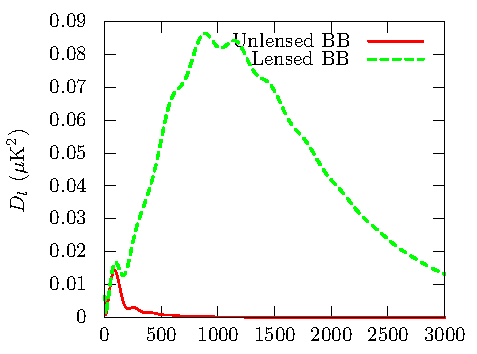
\includegraphics[height=4cm]{plots/excess_BB.pdf}};}
		\uncover<7-8>{%
		\node at (5.5,-0.1) {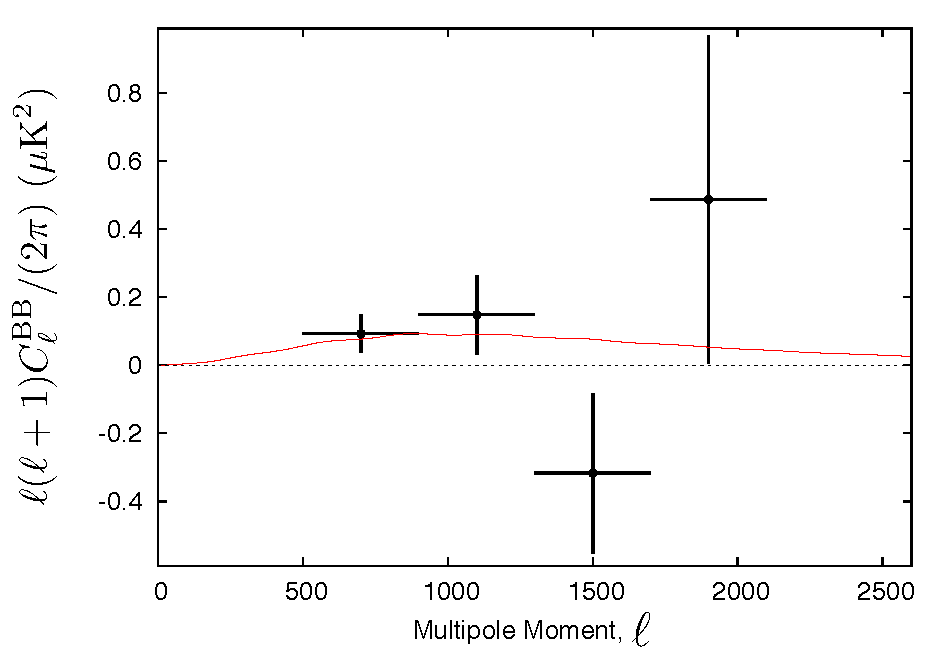
\includegraphics[height=4.2cm,clip,trim=0mm 0mm 0mm -2mm]{plots/polarbear.pdf}};
		\node at (5.4,1.2) {\footnotesize POLARBEAR 2014 $2\sigma$};}

		\uncover<9->{%
		\node at (1.0,0) {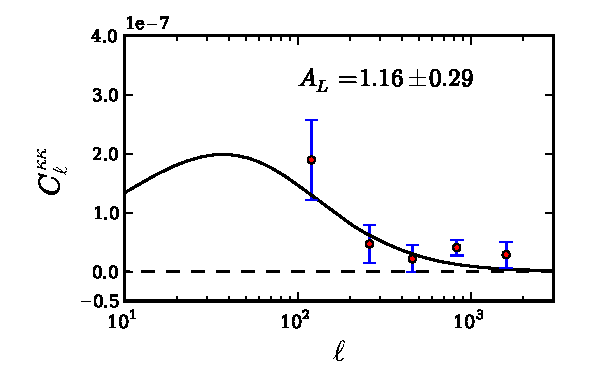
\includegraphics[height=3.7cm,clip,trim=15mm 8mm 0mm 1mm]{plots/act_lens_spec11.pdf}};
		\node at (2,0) {\footnotesize ACT 2011 $4.0\sigma$};}
		\uncover<10->{%
		\node at (6.2,-0.1) {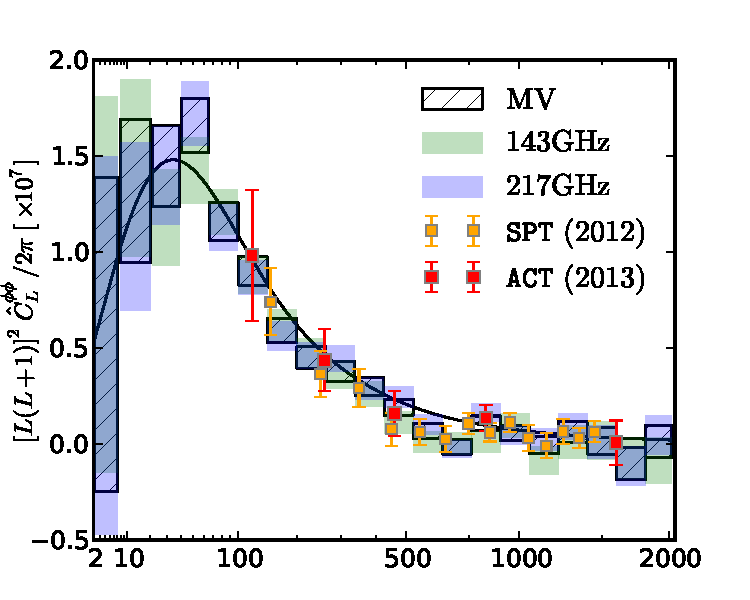
\includegraphics[height=4.2cm,clip,trim=7mm 0mm 0mm 0mm]{plots/planck_lens_spec.pdf}};
		\node at (5.8,-1.5) {\footnotesize Planck 2013 $25\sigma$};}

	\end{tikzpicture}
\end{frame}

\begin{frame}{Observational status}
	\begin{tabular}{lrlrr}
		Type & Year & Dataset & Signif. &arXiv \\
		\rowcolor{red!25}   Cross     & 2007 &WMAP CMB x NRAO galaxies& $3.4\sigma$ &0705.3980  \\
		\rowcolor{green!25} Excess    & 2008 &ACBAR CMB + WMAP CMB    &  $>3\sigma$ &0803.2309  \\
		\rowcolor{green!25} Excess    & 2010 &ACT CMB + WMAP CMB      & $2.8\sigma$ &1009.0847  \\
		\rowcolor{blue!25}  Spectrum  & 2011 &ACT CMB                 & $4.0\sigma$ &1103.2124  \\
		\rowcolor{blue!25}  Spectrum  & 2012 &SPT CMB                 & $6.3\sigma$ &1202.0546  \\
		\rowcolor{red!25}   Cross     & 2012 &SPT CMB x BCS,WISE,Spit.&  $>5\sigma$ &1203.4808  \\
		\rowcolor{red!25}   Cross     & 2012 &ACT CMB x SDSS quasar   & $3.8\sigma$ &1207.4543  \\
		\rowcolor{blue!25}  Spectrum  & 2013 &ACT CMB                 & $4.6\sigma$ &1301.1037  \\
		\rowcolor{red!25}   Cross     & 2013 &SPT CMB x Herchel CIB   &  $>9\sigma$ &1303.5048  \\
		\rowcolor{yellow!25}Imaging   & 2013 &SPT CMB                &$\sim4\sigma$ &1303.5048  \\
		\rowcolor{red!25}   Cross     & 2013 &Planck CMB x NVSS       &  $20\sigma$ &1303.5077  \\
		\rowcolor{blue!25}  Spectrum  & 2013 &Planck CMB              &  $25\sigma$ &1303.5077  \\
		\rowcolor{orange!25}Cross B   & 2013 &SPT CMB x Herschel CIB  & $7.7\sigma$ &1307.5830  \\
		\rowcolor{red!25}   Cross     & 2013 &Planck CMB x tSZ        & $6.2\sigma$ &1312.4525  \\
		\rowcolor{blue!25}  Spectrum (EB) & 2013 &POLARBEAR CMB           & $4.2\sigma$ &1312.6646  \\
		\rowcolor{green!25}  Excess B  & 2014 &POLARBEAR CMB          &$\sim2\sigma$ &1403.2369
	\end{tabular}
\end{frame}

\begin{frame}{(Near) future}
	\begin{center}
		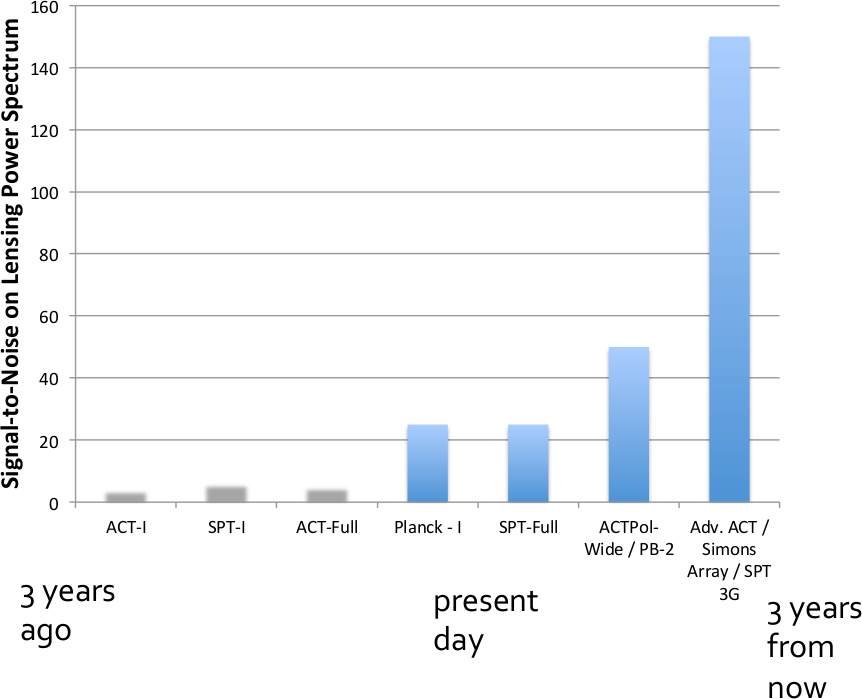
\includegraphics[height=8cm]{plots/cmb_lensing_past_future_blake.png}

		\vspace{-0.5cm}
		{\footnotesize Credit: Blake Sherwin}
	\end{center}
\end{frame}

\end{document}
